%!TEX root = ../thesis.tex
%%--------------------------------------------------------------------------
%% OPENSTACK AND DEVSTACK
%%--------------------------------------------------------------------------


In this chapter we are going to present OpenStack and DevStack giving a brief overview of them and focusing on their components and aspects that concern our thesis topic.

\section{OpenStack}
\label{sec:openstack}
OpenStack is an open-source cloud computing software platform that provides a complete IaaS solution for public and private clouds. Founded by Nasa\footnote{\url{www.nasa.gov} (2015)} and Rackspace Cloud\footnote{\url{www.rackspace.com} (2015)} in 2010 OpenStack is now one of the biggest open-source projects with more than twenty thousand people working on it and more than twenty million code lines. It is a cloud operating system that controls large pools of compute, storage, and networking resources throughout a datacenter, with the possibility to control all of them trough a dashboard and enabling enterprises and service providers to offer on-demand computing resources.\\
One of its main strengths is the modularity that provides the necessary flexibility to design a cloud environment; its core components are:
\begin{description}
	\item[Compute] The service called \textit{Nova} is the primary computing engine and it is used to deploy and manage large number of Virtual Machines.
	\item[Storage] The storage platform, divided in Object Storage (\textit{Swift}) and Block Storage (\textit{Cinder}).
	\item[Network] The service \textit{Neutron} takes care of managing networks. 
	\item[Dashboard] The dashboard \textit{Horizon} provides users  a graphical user interface to access, provision, and automate cloud-based resources.
	\item[Shared Services] Other services, that makes easier to manage the IaaS, such as the Identity Service (\textit{Keystone}), the Image Service (\textit{Glance}), Telemetry (\textit{Ceilometer}), Orchestration (\textit{Heat}) and others.
\end{description}

\begin{figure}[!ht]
\centering{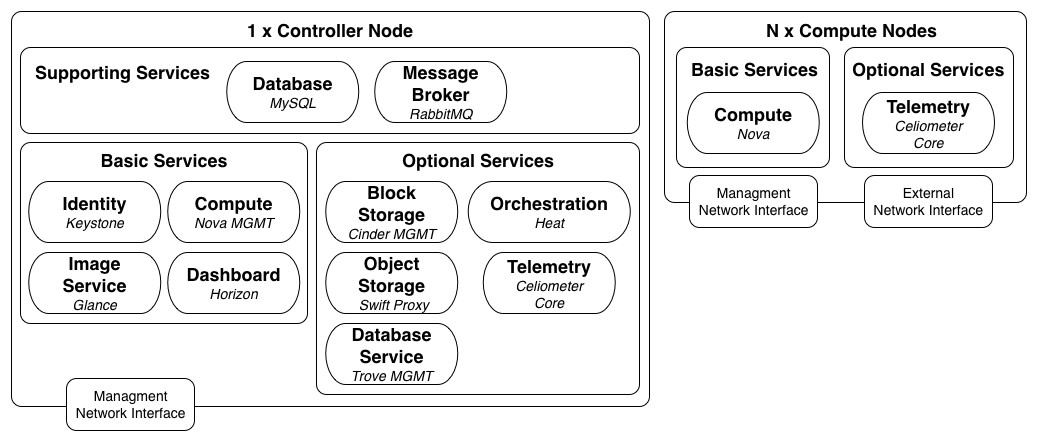
\includegraphics[width=\textwidth]{images/openstack_arch.png}}
\label{fig:openstack_arch}
\caption{The OpenStack architecture}
\end{figure}

\subsection{Nova}
\label{sec:openstack_nova}
OpenStack Compute module, \textit{Nova}, is the core of OpenStack; it takes care to deploy and manage Virtual Machines, place them on physical machines, let them communicate, store their informations on an SQL database and offers both a set of APIs reachable through HTTP requests and a command-line client.

\paragraph{Nova-compute}
\paragraph{Nova-network}
\paragraph{Nova-scheduler}

\subsection{Heat}
\label{sec:openstack_heat}



\section{DevStack}
\label{sec:devstack}

% - devstack
% 	- stack.sh
% 	- unstack.sh
% 	- clean.sh
% 	- 
% 	- dependencies
% 	- configurations local.conf
 